\documentclass[11pt,a4paper]{article}
\usepackage[T1]{fontenc}
\usepackage[utf8]{inputenc}
\usepackage{lmodern,microtype}
\usepackage{amsmath,amssymb,amsthm,mathtools,bm}
\usepackage{booktabs,array,tabularx,longtable}
\usepackage{graphicx,float,caption}
\usepackage{xcolor}
\usepackage[margin=20mm]{geometry}
\usepackage{enumitem,fancyhdr}
\usepackage[hidelinks,unicode=true]{hyperref}
\hypersetup{
 pdftitle={FIN ST190--ST202: Strict-Generated Layers, Selection, and Operational Limits},
 pdfauthor={Krzysztof Żuchowski},
 pdfsubject={Analytical, interval, and computational execution of FIN programs ST190--ST202},
 pdfkeywords={FIN, fractal information, heat semigroup, layered compression, Blackwell sufficiency, spontaneous symmetry breaking, interval continuation, quantum recovery, sample complexity, matrix factor, hidden Markov model}
}
\setlength{\parindent}{0pt}
\setlength{\parskip}{0.48em}
\setlength{\emergencystretch}{2em}
\setlength{\headheight}{14pt}
\setlist[itemize]{leftmargin=1.55em,itemsep=0.14em,topsep=0.2em}
\setlist[enumerate]{leftmargin=1.75em,itemsep=0.14em,topsep=0.2em}
\pagestyle{fancy}\fancyhf{}
\lhead{FIN ST190--ST202}\rhead{Release 10.70}\cfoot{\thepage}
\newtheorem{theorem}{Theorem}[section]
\newtheorem{proposition}[theorem]{Proposition}
\newtheorem{corollary}[theorem]{Corollary}
\newcommand{\proven}{\textcolor{green!40!black}{\textbf{[PROVEN]}}}
\newcommand{\strong}{\textcolor{blue!70!black}{\textbf{[STRONG EVIDENCE]}}}
\newcommand{\conditional}{\textcolor{violet!65!black}{\textbf{[CONDITIONAL]}}}
\newcommand{\openstatus}{\textcolor{red!72!black}{\textbf{[OPEN]}}}
\newcommand{\blocked}{\textcolor{orange!82!black}{\textbf{[BLOCKED]}}}
\newcommand{\boundarymark}{\textcolor{orange!82!black}{\textbf{[BOUNDARY]}}}
\newcommand{\resultbox}[1]{\begin{center}\fcolorbox{blue!60!black}{blue!4}{\parbox{0.92\textwidth}{#1}}\end{center}}

\begin{document}
\pagenumbering{gobble}
\begin{titlepage}
\centering
\vspace*{0.60cm}
{\LARGE\bfseries FIN ST190--ST202\par}
\vspace{0.24cm}
{\Large Strict-Generated Layers, Selection, and Operational Limits\par}
\vspace{0.34cm}
{\large A strict heat-semigroup hierarchy, Blackwell-minimal compression, equivariant positive-feedback selection, 120 validated stationary continuations, generic noncommuting-qubit recovery, selector thermodynamic cost, nonlinear-source nonidentifiability, a certified nuisance boundary, deep-mode sampling lower bounds, exact factor projection, rational hidden-HMM enclosures, interval-certified local-reset no-go results, and an honest external-evidence stop\par}
\vspace{0.65cm}
{\Large Krzysztof \.{Z}uchowski\par}
\vspace{0.16cm}
{\large Independent Researcher --- Fractal Information Theory Project\par}
{\large ORCID: 0009-0002-0909-3613\par}
\vspace{0.45cm}
{\large FIN Release 10.70 --- Version 1.0.0\par}
{\large August 11, 2026\par}
\vfill
\begin{minipage}{0.93\textwidth}
\textbf{Research question.} Can the intuition that our physics is observed on a developed compression layer---with deeper scales visible through intervening fractal-like layers---be made more internal to FIN, rather than imposed as an arbitrary observation channel? What can then be proved about selection, recovery, continuation, sampling, and operational realization?\par
\textbf{Methods.} Conservative matrix semigroups, circulant Fourier analysis, finite Blackwell experiments, equivariant replicator dynamics, outward interval Krawczyk continuation, Bloch-space trace-norm certificates, controlled equilibrium thermodynamics, identifiability theorems, Fisher information and hypothesis-testing bounds, matrix sign functional calculus, exact rational hidden-Markov forward recursion, singular-value perturbation certificates, and executable evidence gates.\par
\textbf{Epistemic rule.} The operator generates the continuous heat family $e^{-tA}$, but it does not select a dyadic schedule or a physical unit of $t$. Repetition is not automatically a geometric fractal; a layer number is not a Planck length; an orbit member chosen by noise is not a canonical selector.\par
\textbf{Repository snapshot.} Audited tracked base commit \texttt{4f388307bdaff902114c020e1adf54307280e7ec}. The working tree contains local research artifacts; the release is accompanied by its own SHA-256 manifest.\par
\textbf{Repository.} \url{https://github.com/hyconiek/Fractal-Nadsoliton-Theory}\par
\textbf{License.} CC BY 4.0.
\end{minipage}
\end{titlepage}
\pagenumbering{arabic}

\begin{abstract}
This report executes programs ST190--ST202. Its central advance is a partial internalization of the layered-compression picture. The strict graph Laplacian $A$ itself generates the positive stochastic semigroup $C(t)=e^{-tA}$. Therefore every supplied increasing sequence of parameters defines a soft hierarchy. For the audited dyadic convention $t_j=2^{j-1}\tau_0$, the composite after $n$ layers is exactly
\[
C^{(n)}=\exp[-(2^n-1)\tau_0A],
\]
and Fourier class $k$ has exact visibility $\exp[-(2^n-1)\tau_0\lambda_k]$. At finite depth all modes are algebraically present; in the infinite-depth limit only the constant mode survives. After eight displayed layers with $\tau_0=1/4$, the smallest nonconstant visibility is about $1.42\times10^{-65}$. This makes ``seeing deeper scales through layers'' a strict spectral-semigroup construction rather than merely a compatible external channel. The decisive limitation remains: neither $\tau_0$, the dyadic schedule, a length ratio, a physical clock, nor the identification of our universe with a particular layer follows from $A$.

ST191 proves the minimal sufficient quotient of a declared twelve-outcome finite experiment. Exactly four likelihood-proportionality classes remain, with an exact stochastic decoder; an over-merge reduces binary total variation from $3/8$ to $1/8$. ST192 constructs a $C_{12}$-equivariant positive-feedback law based on $M=A\circ A$. Uniformity is an exact unstable fixed point, every vertex is locally stable, and exchangeable microscopic perturbations choose several orbit members in twelve seeded runs. The law exhibits spontaneous symmetry breaking but supplies the feedback and perturbation; it cannot canonically label the selected branch and does not discharge QW-2191.

ST193 extends every one of the sixty ST180 signed branches to two further modal slices and interval-certifies all $120/120$ roots. ST194 solves a genuinely noncommuting three-error qubit recovery problem globally over all CPTP recoveries: a trace-norm upper bound is saturated by the polar unitary, giving entanglement fidelity $0.9237212568973701$. ST195 derives a controlled selector's free-energy bound and a convergent quasistatic protocol. ST196 proves that the strict Hessian, $C_{12}$ symmetry, and coercivity cannot determine the magnitude of the degree-twelve coupling $g$.

ST197 certifies a complete $7^3$ nuisance cover to halfwidth $0.00013045$; at $0.00013050$ six cells fail the fixed certificate, which is a method boundary rather than proof of branch loss. ST198 proves that reconstructing a mode attenuated by $2^{-n}$ requires leading sample count proportional to $4^n$; at $n=12$ the displayed estimation lower bound exceeds $4.19\times10^{10}$. ST199 projects noisy Clifford-like generators onto an exact $M_2$ factor by matrix signs. ST200 encloses observed hidden-HMM coefficients through $n=12$ using exact rational forward likelihoods and outward integer-square-root bounds. ST201 upgrades the prior reset evidence to interval-certified no-go theorems for both the four-SWAP span and the complete 60-dimensional corresponding-pair Pauli span. ST202 correctly remains blocked because no external immutable laboratory record exists.

No strict fractal scale law, Planck scale, spacetime projection, canonical selector, physical dimensions, external evidence, legacy-to-strict completion or role transfer, Standard Model, gravity, $L_{\rm total}$, or Theory-of-Everything closure is claimed.
\end{abstract}

\textbf{Status vocabulary.} \proven{} denotes an analytic, exact finite, or outward-interval result in its stated scope. \conditional{} marks a construction using declared added objects. \strong{} denotes numerical evidence. \blocked{} records an unavailable external prerequisite. \boundarymark{} marks a non-implication.

\tableofcontents
\newpage

\section{Frozen mathematical core and kernel discipline}

The strict working kernel remains
\begin{equation}
W_{xx}=0,\qquad
W_{xy}=\frac{\cos(0.18575d(x,y)+0.16250)}{1+d(x,y)^{9/5}}\quad(x\ne y),
\qquad A=sI-W,
\label{eq:strict}
\end{equation}
on the cycle $C_{12}$, where
\[
s=2\sum_{d=1}^{5}W(d)+W(6),\qquad
\langle f,Af\rangle=\frac12\sum_{x,y}W_{xy}|f_x-f_y|^2\ge0.
\]
The explicit diagonal convention $W_{xx}=0$ is essential: the quoted row sum and Laplacian identity apply to the off-diagonal interaction.

The legacy ontological kernel remains an intermediate bridge kernel. Equation~\eqref{eq:strict} is the later enriched strict working kernel; no legacy electroweak, electromagnetic, gravity-hierarchy, or other physical role is transferred to it without a completion map and a separate role-transfer theorem. The nadsoliton remains the primordial fractal information in a solitonic state. There is no lower informational substrate beneath it.

\resultbox{\textbf{Central interpretation after ST190.} The strict operator does generate a continuous family of possible compression layers, namely $e^{-tA}$. It does not generate a preferred discrete scale schedule. Consequently the theory now contains a rigorous \emph{layer mechanism} but not yet a rigorous \emph{fractal scale law}. Our observed physics may be modeled as statistics at one effective layer, but the layer index, dimensional scale, instruments, and empirical identification remain additional data.}

\section{Outcome matrix}
\small
\begin{longtable}{@{}p{0.06\textwidth}p{0.23\textwidth}p{0.33\textwidth}p{0.30\textwidth}@{}}
\toprule ID & Target & Result & Boundary\\\midrule\endfirsthead
\toprule ID & Target & Result & Boundary\\\midrule\endhead
ST190 & Internal hierarchy candidate & \proven{} strict heat semigroup and exact dyadic visibility & Schedule and scale supplied\\
ST191 & Minimal carrier quotient & \proven{} four-class Blackwell-minimal statistic & Experiment/preparations supplied\\
ST192 & Spontaneous pointer selection & \conditional{} equivariant feedback; uniform unstable, vertices stable & Feedback/noise supplied; no canonical label\\
ST193 & Branch continuation & \proven{} $120/120$ further modal slices certified & Not global pseudo-arclength atlas\\
ST194 & Noncommuting recovery & \proven{} global CPTP optimum for declared channel & Positive polar orientation, qubit scope\\
ST195 & Selector-control cost & \proven{} free-energy bound and convergent protocol & Bath, field, vertex and control supplied\\
ST196 & Source of $g$ & \proven{} infinite-family nonidentifiability & Extra nonlinear datum required\\
ST197 & Nuisance boundary & \proven{} cover to $1.3045\times10^{-4}$ & Upper failure is method-specific\\
ST198 & Deep-mode samples & \proven{} Fisher/Pinsker lower bounds, leading $4^n$ growth & Observation law supplied\\
ST199 & Exact factor recovery & \proven{} sequential sign projection; exact factor & Not globally nearest joint factor\\
ST200 & Observed-HMM rate & \proven{} exact-rational finite-$n$ intervals & Asymptotic rate open\\
ST201 & Local reset & \proven{} interval full rank in 4D and 60D spans & Static corresponding-pair scope\\
ST202 & External execution & \blocked{} gate correctly refuses promotion & No external record or custody\\
\bottomrule
\end{longtable}
\normalsize

\section{ST190: a strict-generated soft hierarchy}

Because $W_{xy}\ge0$ for all audited distances and every row of $A$ sums to zero, $-A$ is a conservative Metzler generator. Hence
\[
C(t)=e^{-tA},\qquad t\ge0,
\]
is entrywise nonnegative, row-stochastic, symmetric, and contractive.

\begin{theorem}[Strict heat hierarchy]
Let $t_1,\ldots,t_n\ge0$. Then
\[
C(t_n)\cdots C(t_1)=C\!\left(\sum_{j=1}^nt_j\right).
\]
For a strict Fourier eigenvector $v_k$ with $Av_k=\lambda_kv_k$, its layer visibility is
\[
\frac{\|C(t_n)\cdots C(t_1)v_k\|}{\|v_k\|}
=\exp\!\left[-\lambda_k\sum_{j=1}^nt_j\right].
\]
For every finite total parameter the map is invertible. As the total tends to infinity, all classes with $\lambda_k>0$ vanish and only $\ker A$ remains.
\end{theorem}

The audited convention chooses $t_j=2^{j-1}\tau_0$ with $\tau_0=1/4$, so
\[
C^{(n)}=\exp[-(2^n-1)\tau_0A].
\]
The seven Fourier-class eigenvalues are approximately
\[
0, 0.754121, 1.577050, 1.961407, 2.199569, 2.298606, 2.342182.
\]
After eight layers the total parameter is $63.75$. The most attenuated class has visibility $1.42465\times10^{-65}$, while the numerical semigroup composition error is $1.15\times10^{-14}$.

\begin{figure}[H]\centering
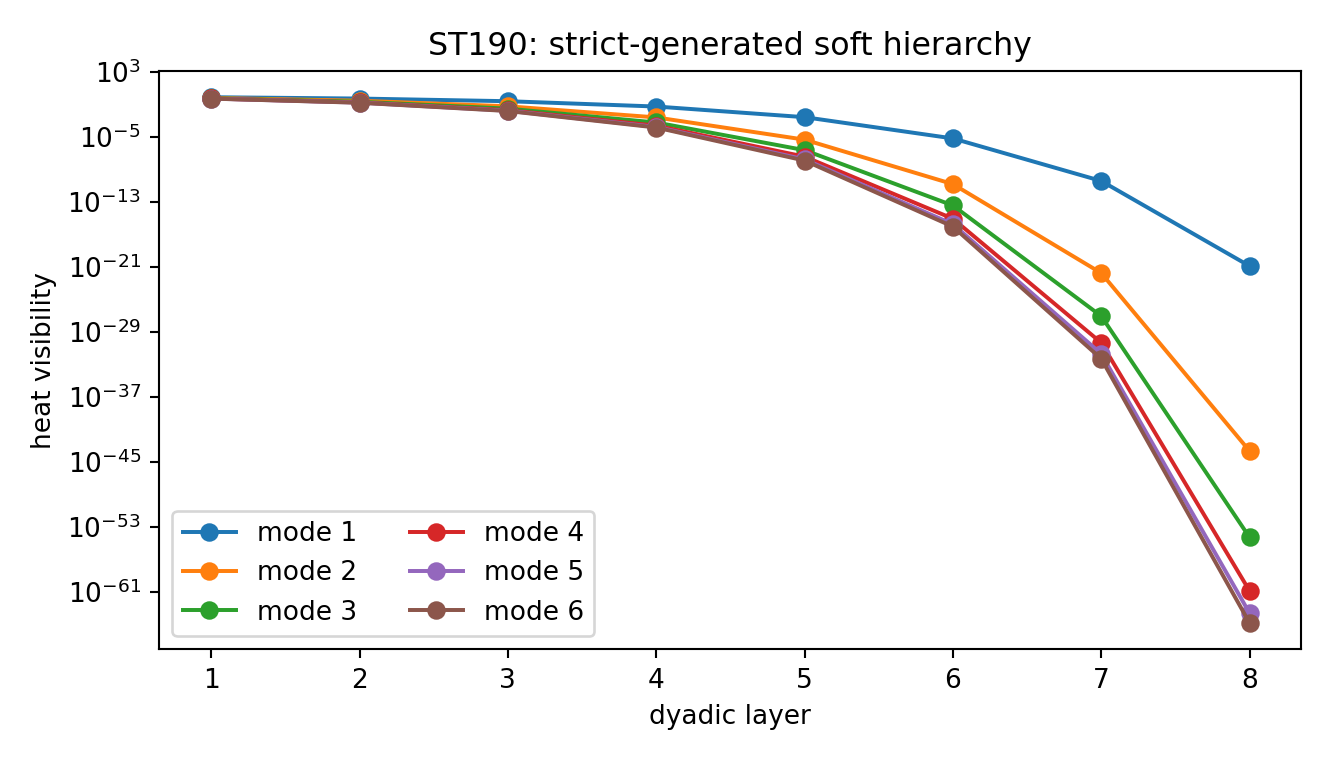
\includegraphics[width=.76\textwidth]{FIN_ST190_ST202_Figures/st190_heat_hierarchy.png}
\caption{ST190. Exact spectral visibility under a supplied dyadic schedule of strict heat channels. The construction becomes practically rank one long before any mode is algebraically deleted.}
\end{figure}

\boundarymark{} A continuous semigroup does not select the set $\{\tau_0,2\tau_0,4\tau_0,\ldots\}$. The dyadic pattern is self-similar because it was chosen so. A genuine FIN fractal law would have to derive a preferred refinement endofunctor or scale character and prove why its ratio is selected. Moreover, the transformation $(A,t)\mapsto(cA,t/c)$ preserves $e^{-tA}$, so the frequency/decay parameter alone does not generate seconds.

\section{ST191: Blackwell-minimal information visible through a layer}

For a finite experiment with hypotheses $h$ and fine outcomes $x$, write the likelihood column
\[
\ell_x=(p(x|h))_h.
\]
A deterministic coarse statistic groups outcomes into fibers.

\begin{theorem}[Minimal sufficient finite quotient]
A deterministic statistic is Blackwell sufficient exactly when all likelihood columns inside each fiber are proportional. The partition into maximal proportionality classes is the unique minimal sufficient deterministic quotient, up to relabeling.
\end{theorem}

\emph{Proof sketch.} If $\ell_x=r_xm_g$ on a fiber $g$, the conditional distribution $r_x/\sum_{y\in g}r_y$ is independent of the hypothesis and defines a stochastic decoder. Conversely, a hypothesis-independent decoder forces every fine likelihood in a fiber to factor through the same coarse likelihood, hence the columns are proportional. Minimality follows because inequivalent columns cannot share a sufficient fiber.\hfill$\square$

The exact rational example has twelve outcomes arranged in four triples. It has precisely the four classes
\[
\{0,1,2\},\ \{3,4,5\},\ \{6,7,8\},\ \{9,10,11\}.
\]
Uniform redistribution inside each triple is an exact stochastic decoder. Merging the first two inequivalent classes decreases total variation between two declared hypotheses from
\[
\frac38\quad\hbox{to}\quad\frac18.
\]

This sharpens the earlier range/kernel criterion: the information surviving a layer depends not only on the channel, but on the preparation/decision experiment relative to which sufficiency is defined. There is no single smallest quotient independent of the operational family.

\section{ST192: symmetry as a reservoir of branches, not a feedback law}

To test whether a symmetric foundation can generate a concrete branch after a perturbation, define
\[
M=A\circ A,
\qquad
\dot p_i=\gamma p_i\bigl[(Mp)_i-p^TMp\bigr]
\]
on the probability simplex. Here $\circ$ denotes entrywise multiplication.

\begin{theorem}[Constructed equivariant selector dynamics]
The law is $C_{12}$-equivariant and preserves positivity and total probability. The uniform state $u=(1/12,\ldots,1/12)$ is an exact fixed point. On the tangent space $\sum_i\delta p_i=0$, its linear growth rates are the nonconstant Fourier eigenvalues of $M$ divided by $12$. All are positive in the strict instance; the smallest is $0.1979393067\gamma$. Every vertex is locally attracting, with displayed minimum invasion margin $2.5357337274\gamma$.
\end{theorem}

Twelve exchangeable Gaussian perturbations of size $2\times10^{-3}$ select seven different vertices; every final largest probability exceeds $0.99999999999$.

\begin{figure}[H]\centering
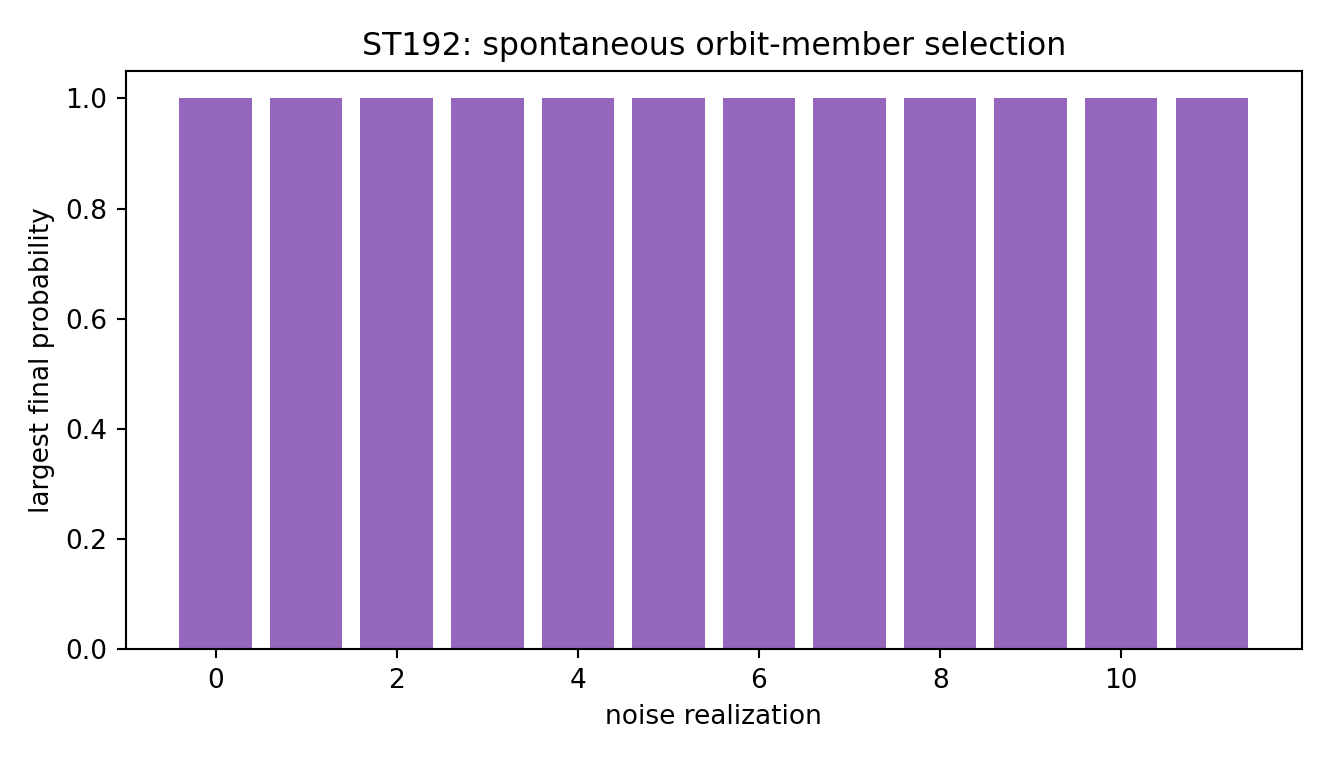
\includegraphics[width=.73\textwidth]{FIN_ST190_ST202_Figures/st192_replicator_selection.png}
\caption{ST192. Positive feedback amplifies a small perturbation into a nearly pure orbit member. The labels vary because the unperturbed law has no preferred label.}
\end{figure}

This validates the refined intuition
\[
\text{symmetry}\to\text{degenerate possibilities}\to\text{perturbation}
\to\text{positive feedback}\to\text{stable branch}.
\]
It also proves why symmetry itself is not positive feedback. Without the added replicator law the uniform state does not move; with no perturbation it remains there exactly. The construction is therefore a mechanism candidate, not a strict selector source. It chooses an orbit member but cannot provide an automorphism-invariant meaning to ``vertex $+1$'' rather than ``vertex $-1$.'' QW-2191 remains open.

\section{ST193 and ST197: validated continuation and its method boundary}

\subsection{Two further slices on every ST180 branch}

ST180 certified sixty nonuniform stationary roots at signed modal coordinate $\epsilon=\pm10^{-3}$. ST193 uses each root as a predictor and continues it to
\[
\epsilon=\pm2\times10^{-3},\qquad \epsilon=\pm5\times10^{-3}.
\]

\begin{theorem}[Validated modal ladder]
All $60\times2=120$ new square systems pass outward Krawczyk inclusion. Thus each accepted box contains exactly one stationary root for every strict operator in the transcendental interval enclosure. The smallest inclusion margin is
\[
2.9844724869\times10^{-7}>0.
\]
\end{theorem}

This establishes longer local branches than ST180. It is not pseudo-arclength continuation: fixed modal slices can miss turns, reconnecting branches, or off-sector solutions.

\subsection{A sharp fixed-grid certificate transition}

For the three nuisance coordinates, the equal $7^3$ cover passes at global halfwidth
\[
h_-=0.00013045
\]
in all 343 cells, with minimum inclusion margin $5.3522\times10^{-7}$. At
\[
h_+=0.00013050,
\]
only 337 cells pass and the lowest margin is $-1.0287\times10^{-6}$.

\begin{theorem}[Fixed-cover boundary]
The stationary root is uniquely continued throughout the complete cube of halfwidth $h_-$. The fixed $7^3$ Krawczyk construction does not certify the full cube at $h_+$.
\end{theorem}

The interval $[h_-,h_+]$ has width $5\times10^{-8}$. It brackets a \emph{method boundary}, not a mathematical branch boundary. Smaller adaptive cells may restore inclusion beyond $h_+$.

\section{ST194: global recovery of three noncommuting qubit errors}

Let three unitary errors act as Bloch rotations $R_a\in SO(3)$ with probabilities $q_a$, and let
\[
T=\sum_aq_aR_a.
\]
The three displayed rotations have pairwise commutator norms $0.5565$, $0.8559$, and $0.9360$, so they are genuinely noncommuting.

\begin{theorem}[Trace-norm recovery certificate]
For every positive trace-preserving qubit recovery with Bloch linear part $S$,
\[
\|S\|_2\le1,
\qquad
F_e(\mathcal R\circ\mathcal E)=\frac{1+\operatorname{tr}(ST)}4
\le\frac{1+\|T\|_*}{4}.
\]
If the orthogonal polar factor of $T$ has determinant $+1$, a unitary recovery realizes it and saturates the bound. It is therefore globally optimal over all CPTP recoveries.
\end{theorem}

\emph{Justification of the contraction bound.} A positive trace-preserving qubit map sends the Bloch ball into itself. Comparing the images of opposite pure states gives $\|Sr\|\le1$ for every unit vector $r$. Von Neumann's trace inequality then gives the upper bound. Positive polar orientation makes the maximizing contraction a physical rotation.\hfill$\square$

For the declared channel, the singular values of $T$ are
\[
0.9798239054,quad0.8676186084,quad0.8474425138,
\]
and the optimum is
\[
\boxed{F_e^*=0.9237212568973701}.
\]
The recorded primal--upper gap is zero at floating precision. This replaces the proposed SDP calculation by a stronger analytic certificate in the positive-orientation qubit class. Negative polar orientation and nonunital channels require a separate optimization.

\section{ST195 and ST196: pricing a selector and proving that \texorpdfstring{$g$}{g} is not sourced}

\subsection{Thermodynamic control cost}

Supply a preferred vertex with controlled energies $E_0=0$, $E_j=b$ for $j\ne0$, in units where $\beta=1$. Its equilibrium probability is
\[
p_0(b)=\frac1{1+11e^{-b}}.
\]
The reversible free-energy change from the uniform zero-field state is
\[
\Delta F=-\log\frac{1+11e^{-b}}{12}.
\]

\begin{theorem}[Selector work bound]
Every isothermal implementation of the supplied field obeys $W\ge\Delta F$. If $b$ is divided into $m$ increments and the state equilibrates before every increment, then
\[
W_m=\sum_{j=0}^{m-1}\bigl[1-p_0(jb/m)\bigr]\frac bm
\searrow\Delta F.
\]
The dimensionless dissipation $W_m-\Delta F$ is positive and converges to zero.
\end{theorem}

For $b=3$, $p_0=0.6461376869$, $\Delta F=2.0481639895$, and 512 steps leave dissipation $0.0016484053$. The displayed protocol first reaches dissipation budgets $0.1,0.05,0.01,0.005$ at 16, 32, 128, and 256 steps respectively.

\begin{figure}[H]\centering
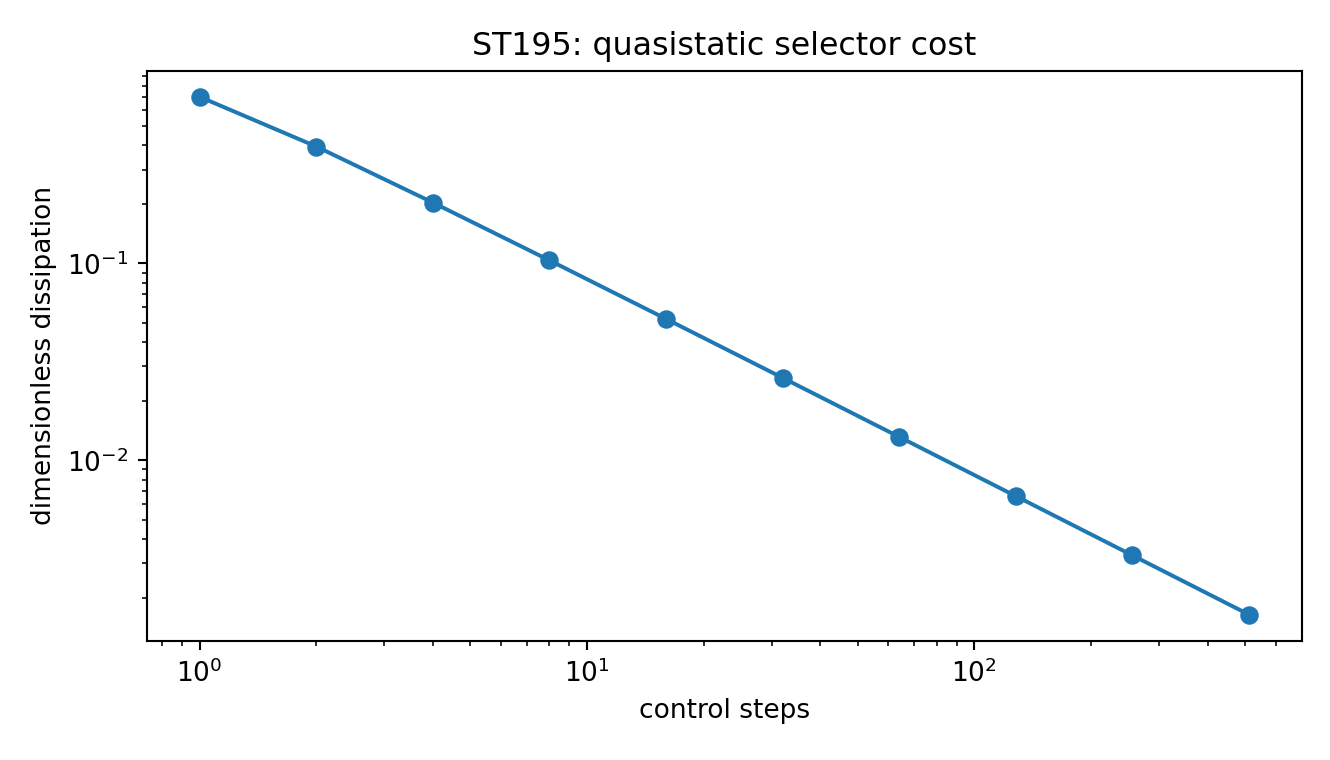
\includegraphics[width=.72\textwidth]{FIN_ST190_ST202_Figures/st195_selector_cost.png}
\caption{ST195. Added control can make selection arbitrarily close to reversible, but the selected vertex and field remain resources.}
\end{figure}

\subsection{No source theorem for the degree-twelve coupling}

Consider
\[
V_g(\psi)=\frac12\psi^TA\psi+\frac g{12}\sum_{j=0}^{11}\psi_j^{12}.
\]

\begin{theorem}[Nonlinear-source nonidentifiability]
For every $g>0$, $V_g$ has the same Hessian $A$ at the origin, the same $C_{12}$ symmetry, and is coercive. Nevertheless
\[
\frac{\partial^{12}V_g}{\partial\psi_j^{12}}(0)=11!g.
\]
Therefore $A$, strict linear response, symmetry, and boundedness below determine only the class $g>0$, not its magnitude.
\end{theorem}

This is an infinite-family obstruction. ST183's response estimators identify $g$ if a nonlinear response is supplied, but identification from data is not derivation from the strict core.

\section{ST198: seeing a deep mode requires exponentially many samples}

Let a deep binary contrast $\delta$ be attenuated to $a=\sigma\delta$, producing probabilities $1/2\pm a$.

\begin{theorem}[Estimation and testing lower bounds]
The Fisher information per multinomial sample for $\delta$ is
\[
I_1(\delta)=\frac{4\sigma^2}{1-4\sigma^2\delta^2}.
\]
Every unbiased estimator with standard deviation at most $\varepsilon$ satisfies
\[
N\ge\frac{1}{I_1(\delta)\varepsilon^2}.
\]
For testing $+\delta$ against $-\delta$ with equal-prior error at most $\alpha$, Pinsker's inequality gives the necessary condition
\[
N\ge\frac{2(1-2\alpha)^2}{D_{\rm KL}(P_+\|P_-)}.
\]
The same information expression holds for independent Poisson category counts when $N$ denotes expected total count.
\end{theorem}

For the soft visibility $\sigma_n=2^{-n}$, the leading burden grows as $\sigma_n^{-2}=4^n$. With $\delta=0.05$ and target standard deviation $0.01$, the lower bound rises from $2475$ samples at $n=0$ to
\[
41{,}943{,}039{,}975
\]
at $n=12$. The corresponding necessary count in the displayed $5\%$ testing bound is $1{,}358{,}954{,}496$.

\begin{figure}[H]\centering
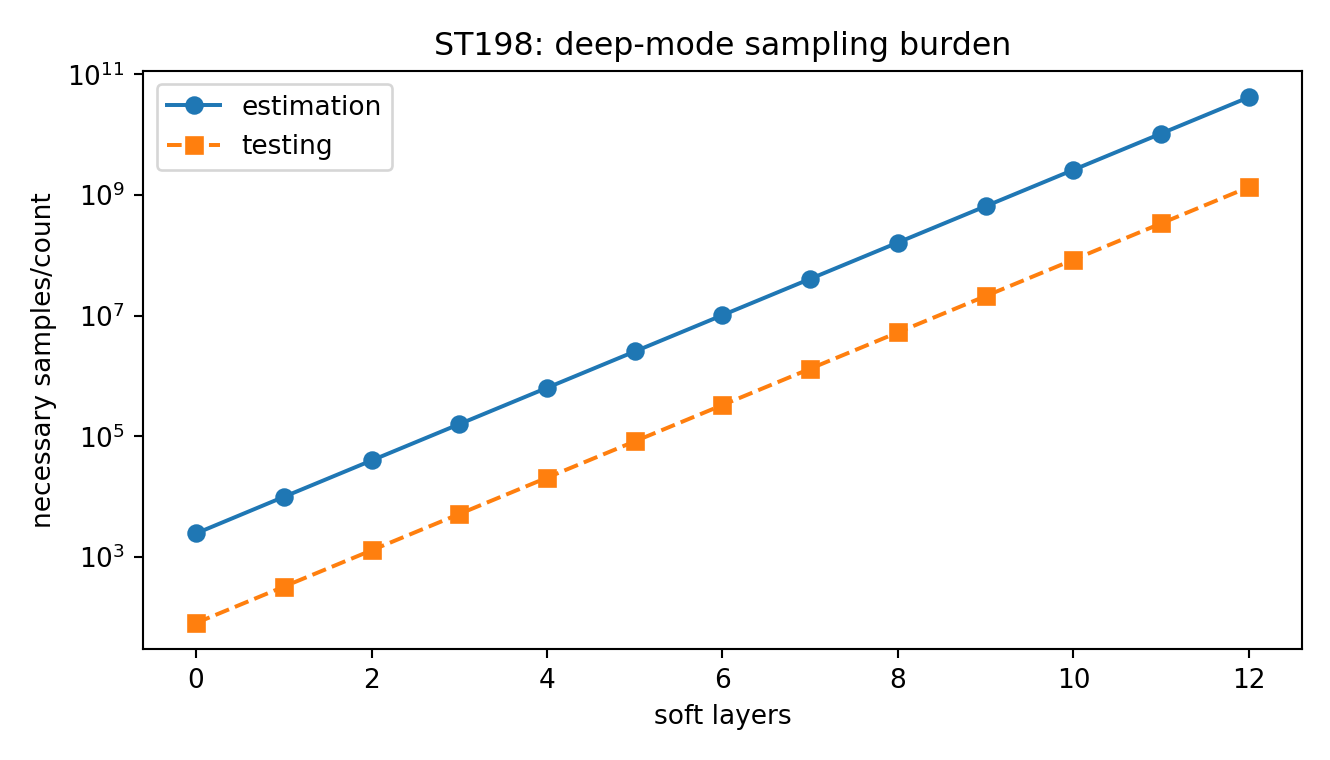
\includegraphics[width=.74\textwidth]{FIN_ST190_ST202_Figures/st198_sampling_bounds.png}
\caption{ST198. Exponential statistical cost is the operational meaning of a deep mode becoming only a faint shadow rather than exactly disappearing.}
\end{figure}

This strengthens the layer interpretation: even an invertible finite-depth map can make fine structure empirically inaccessible. It does not show that an actual detector obeys this binary or Poisson model.

\section{ST199: from a noisy subspace to an exact matrix factor}

Let $X_0,Z_0$ be noisy Hermitian approximations to two anticommuting involutions. Define
\[
X=\operatorname{sign}(X_0),\qquad
Z_o=\frac12(Z_0-XZ_0X),\qquad
Z=\operatorname{sign}(Z_o).
\]

\begin{theorem}[Sequential exact factor projection]
If $X_0$ is invertible, $X$ is the unique nearest Hermitian involution to $X_0$ in Frobenius norm. If $Z_o$ is invertible, then
\[
X^2=Z^2=I,\qquad XZ+ZX=0.
\]
With balanced positive/negative multiplicities, $X$ and $Z$ generate a copy of $M_2$ and their commutant is another $M_2$.
\end{theorem}

For generator-noise levels $0.001$, $0.003$, $0.01$, and $0.03$, the displayed sign gaps remain above $0.9835$. All four projected pairs have generated-algebra dimension four, commutant dimension four, and involution/anticommutation residuals below $2.5\times10^{-15}$.

This constructs an exact algebra from noisy data. It does not prove that the sequential result is the globally nearest \emph{joint} factor pair, remove local-unitary gauge, recover instrument labels, or establish physical subsystems.

\section{ST200: exact-rational finite hidden-HMM enclosures}

The observed Hellinger coefficient is
\[
Z_n=\sum_{y^n}\sqrt{P_0(y^n)P_1(y^n)}.
\]
Both hidden transition and emission probabilities in the declared model are rational. ST200 computes every forward likelihood exactly as a rational number. For $r=a/b$, it bounds the square root by
\[
\frac{\lfloor D\sqrt{ab}\rfloor}{bD}
\le\sqrt{\frac ab}\le
\frac{\lfloor D\sqrt{ab}\rfloor+1}{bD},
\qquad D=10^{35}.
\]

\begin{theorem}[Finite observed-rate enclosure]
Summing these exact rational bounds over all $2^n$ records gives an outward rational interval for $Z_n$. Monotonicity of $-\log$ gives an outward interval for $-n^{-1}\log Z_n$.
\end{theorem}

At $n=12$ the coefficient is enclosed, after outward binary rounding, by
\[
[0.00012412149508879994, 0.00012412149508880000],
\]
and the finite rate by
\[
[0.7495208060788203, 0.7495208060788207].
\]
The underlying rational interval is much narrower than the displayed double interval.

\begin{figure}[H]\centering
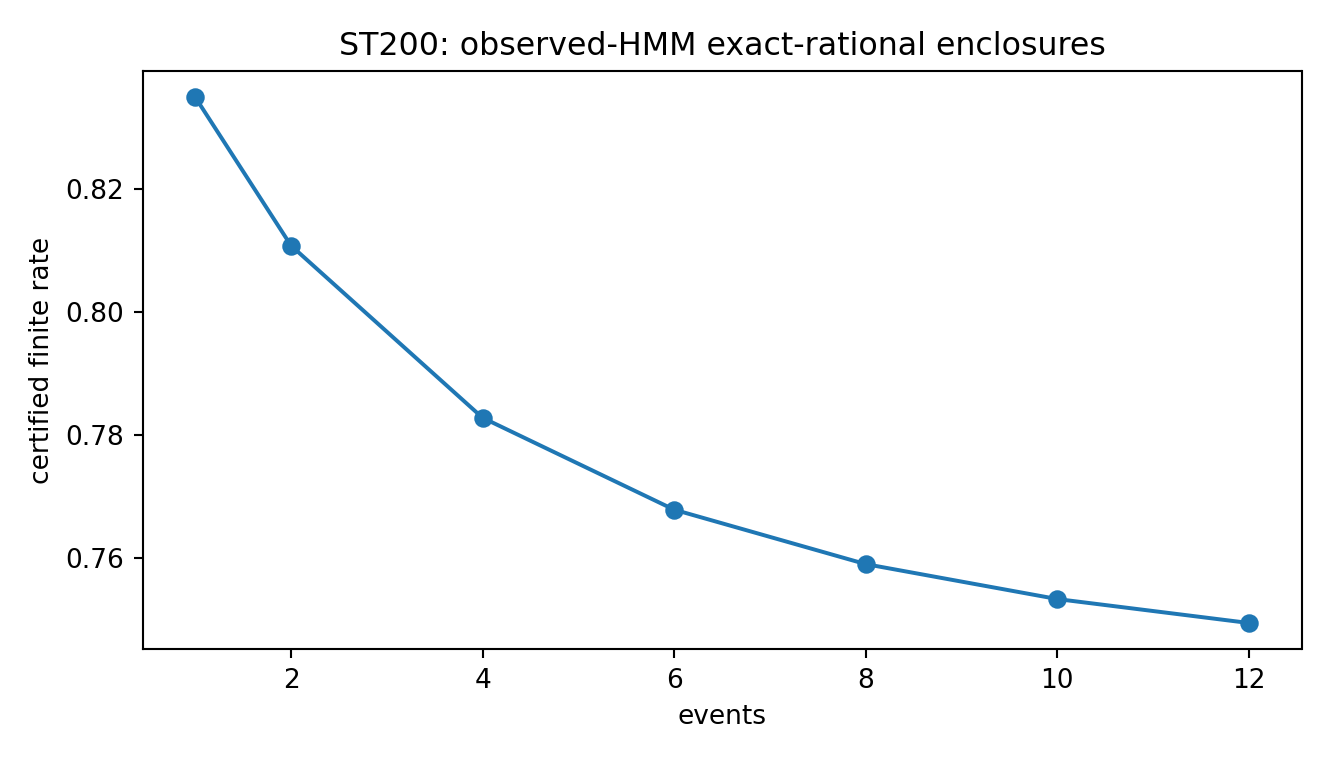
\includegraphics[width=.72\textwidth]{FIN_ST190_ST202_Figures/st200_hmm_intervals.png}
\caption{ST200. Certified finite observed-process rates through complete enumeration of $4096$ records at $n=12$.}
\end{figure}

This removes the finite floating uncertainty noted in ST187. It does not prove existence or value of the exact asymptotic rate; a rigorous transfer operator on belief-pair space remains open.

\section{ST201: an interval-certified static local-reset no-go}

Embed the strict twelve-level Hamiltonian in a sixteen-level four-qubit register and set
\[
H_{\rm tot}=H\otimes I+I\otimes H.
\]
For generators $G_j$, define the commutator matrix whose $j$th column is the vectorization of $[H_{\rm tot},G_j]$.

The outward strict-kernel enclosure has maximum entry radius
\[
\delta_A=6.6613381478\times10^{-16}.
\]
If $G_j$ is unitary, the Frobenius error of one commutator column is bounded by $192\delta_A$. Thus for $m$ columns the singular-value perturbation is at most $192\sqrt m\,\delta_A$.

\begin{theorem}[Static corresponding-pair reset obstruction]
The four pairwise-SWAP commutator columns have a shifted-Cholesky certificate with smallest singular value greater than
\[
14.1421355883.
\]
The full sixty-dimensional span of all nonidentity two-qubit Pauli generators on the four corresponding system--bath qubit pairs has a corresponding certified smallest singular value greater than
\[
6.3245552412.
\]
Consequently neither span contains a nonzero static generator commuting with $H_{\rm tot}$.
\end{theorem}

\begin{figure}[H]\centering
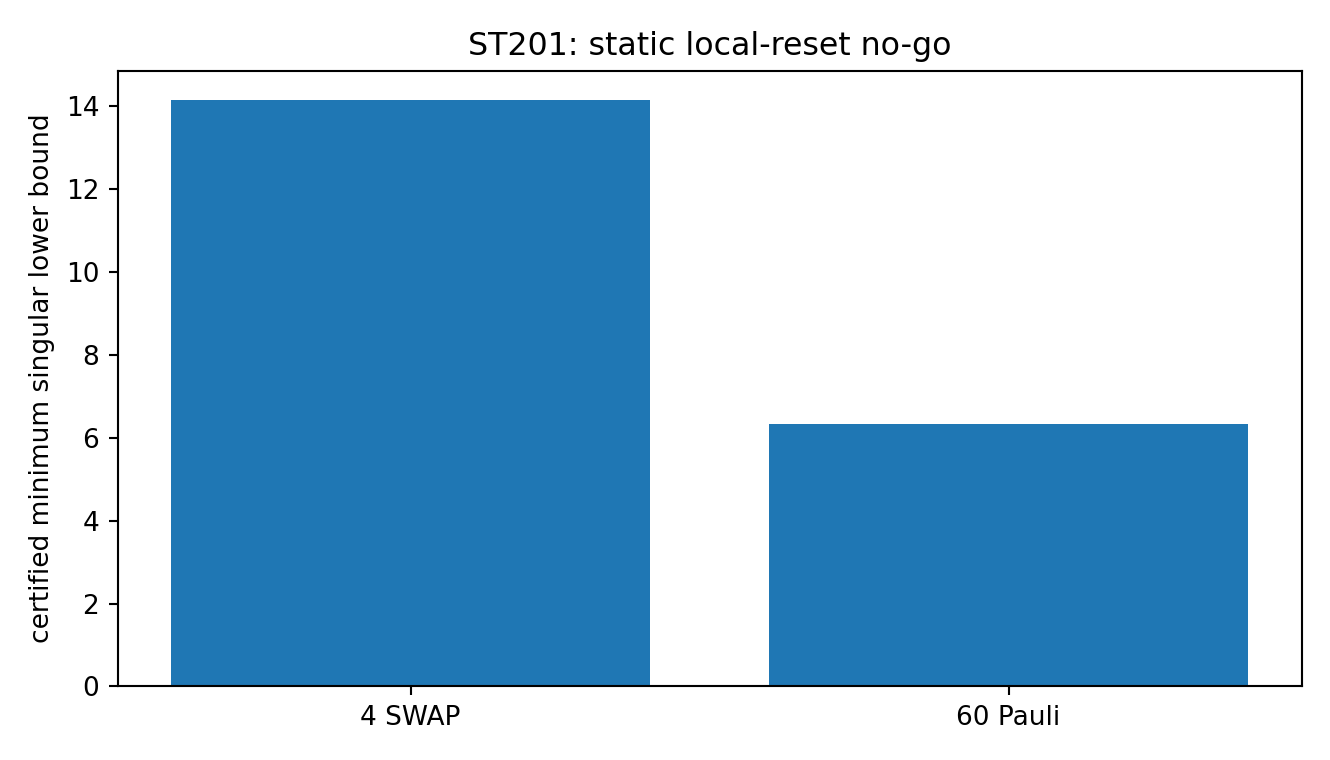
\includegraphics[width=.69\textwidth]{FIN_ST190_ST202_Figures/st201_reset_rank.png}
\caption{ST201. Positive interval/shifted-Cholesky lower bounds close both declared static local-generator spans.}
\end{figure}

This promotes the ST188 four-generator evidence and substantially enlarges its scope. It remains encoding- and ansatz-specific. Time-dependent controls, noncorresponding edges, ancillas, and higher-locality interactions are not excluded. Global register SWAP remains an exact energy-conserving construction.

\section{ST202: the scientifically correct result is ``not executed''}

The immutable-record interface still passes its synthetic tamper test. However, no genuinely external event path, frozen holdout hash supplied by an independent registrar, calibration hash, distinct verified human roles, custody attestation, or laboratory-execution attestation was supplied.

\begin{theorem}[Evidence gate]
Under the declared schema, absence of the external provenance atoms makes the physical-execution predicate false. No local program can generate those facts without changing their meaning.
\end{theorem}

Therefore ST202 is \blocked{}, not failed and not simulated. This is a methodological result: a theory package can validate syntax and hashes locally, but it cannot manufacture independent evidence.

\section{Synthesis: are we observing lower scales through fractal layers?}

The new results support the following precise conditional architecture:
\[
\text{primordial nadsoliton information}
\xrightarrow{e^{-t_1A}}
\text{effective layer 1}
\xrightarrow{e^{-t_2A}}\cdots
\xrightarrow{e^{-t_nA}}
\text{accessible statistics}.
\]

Three distinct mathematical notions must not be conflated:

\begin{enumerate}
\item \textbf{Existence at depth.} A nonconstant mode exists in the deep state.
\item \textbf{Algebraic visibility.} At finite heat depth its multiplier is nonzero, so exact noiseless inversion exists.
\item \textbf{Operational visibility.} Finite samples and noise make inversion feasible only if the multiplier is not too small; ST198 quantifies the cost.
\end{enumerate}

Thus our effective physics could, as a mathematical hypothesis, be a view of deeper information through a developed layer. Lower scales would appear as attenuated or quotiented shadows. The same picture is compatible with renormalization, diffusion distance, sufficient statistics, and noisy inverse problems, but compatibility is not equivalence.

\subsection{What would make the hierarchy genuinely fractal?}

At least one additional theorem must produce:
\begin{enumerate}
\item a preferred refinement/coarse-graining endofunctor or scale map;
\item an internally selected ratio or fixed-point law between levels;
\item a rule transporting states, observables, and dynamics coherently across levels;
\item a dimension/clock map connecting a level parameter to physical length or duration;
\item preparations and instruments that identify which quotient is empirically accessible.
\end{enumerate}

Without items 1--3, ``fractal'' means only repeated construction. Without item 4, no layer is a Planck layer. Without item 5, no layer is our observed physics.

\subsection{Combined selector lesson}

ST192 gives a genuine mechanism of orbit selection after a perturbation. ST195 prices an externally controlled selector. Together they show:
\[
\text{symmetric possibilities}+\text{amplifying dynamics}+\text{fluctuation}
\Longrightarrow\text{one realized branch}.
\]
They do not show:
\[
A\Longrightarrow\text{canonical branch label}.
\]
The first statement is spontaneous symmetry breaking in a constructed dynamics; the second is the unresolved strict selector theorem.

\subsection{What was falsified or bounded}

\begin{itemize}
\item The strict operator does not select the dyadic hierarchy parameter used in ST190.
\item Symmetry alone does not create positive feedback; the uniform state remains fixed until a feedback law and perturbation are supplied.
\item Strict linear data, symmetry, and coercivity do not determine the nonlinear magnitude $g$.
\item A finite-depth mode can be algebraically present yet statistically inaccessible because sample cost grows as the inverse squared visibility.
\item The static local-reset obstruction persists after enlarging the generator class from four SWAPs to sixty two-qubit Pauli terms.
\item Exact finite hidden-HMM arithmetic does not by itself determine the infinite-record exponent.
\item Local software cannot turn synthetic records into external laboratory evidence.
\end{itemize}

\section{Recommended programs ST203--ST217}

\begin{longtable}{@{}p{0.08\textwidth}p{0.12\textwidth}p{0.72\textwidth}@{}}
\toprule Program & Priority & Executable target\\\midrule\endfirsthead
\toprule Program & Priority & Executable target\\\midrule\endhead
ST203 & 1 & Classify strict-generated completely positive semigroup hierarchies and test whether any schedule is selected internally.\\
ST204 & 2 & Derive the lattice of Blackwell-equivalent FIN experiments across preparation and instrument families.\\
ST205 & 3 & Replace injected symmetric noise in ST192 by a strictly typed endogenous fluctuation source, or prove a source no-go.\\
ST206 & 4 & Perform validated pseudo-arclength continuation and isolate global branch collisions beyond the ST193 slices.\\
ST207 & 5 & Extend the recovery certificate to negative polar orientation and nonunital qubit channels.\\
ST208 & 6 & Solve finite-time entropy-production optimal control under a frozen generator-rate budget.\\
ST209 & 7 & Classify the minimal additional response datum that identifies $g$ while remaining carrier-invariant.\\
ST210 & 8 & Use adaptive interval subdivision beyond the fixed-grid ST197 certificate boundary.\\
ST211 & 9 & Derive minimax bounds for simultaneous deep Fourier modes under correlated counts.\\
ST212 & 10 & Prove or refute global nearest-joint-factor uniqueness beyond the sequential ST199 projection.\\
ST213 & 11 & Construct a rigorous interval transfer operator for the exact asymptotic observed-HMM rate.\\
ST214 & 12 & Search time-dependent energy-conserving local reset controls outside the static ST201 span.\\
ST215 & 13 & Test whether a refinement tower induces an effective metric through diffusion distance without a dimensional anchor.\\
ST216 & 14 & Formalize the distinction between viewing lower scales through layers and reconstructing them from sufficient statistics.\\
ST217 & 15 & Execute the immutable-record gate only after genuine laboratory data, calibration, and independent custody are supplied.\\
\bottomrule
\end{longtable}

The greatest conceptual leverage lies in ST203: ST190 supplies a strict-generated continuous layer family, and the remaining question is whether a preferred self-similar schedule can emerge without being inserted. ST205 is the highest-value selector program. ST206, ST210, ST213, and ST214 are the strongest proof-grade computational continuations.

\section{Reproducibility and claim ledger}

The release package contains:
\begin{itemize}
\item \texttt{fin\_st190\_st202\_research.py}: all thirteen programs and six figures;
\item \texttt{test\_fin\_st190\_st202.py}: 27 serialized and live tests;
\item \texttt{FIN\_ST190\_ST202\_Results.json} and thirteen specialized JSON packets;
\item \texttt{FIN\_ST190\_ST202\_Summary.csv};
\item this source report, compiled PDF, release description, and SHA-256 manifest.
\end{itemize}

The seeded components use seed \texttt{20260811}. The Blackwell quotient is exact rational. The ST193 and ST197 certificates use outward interval arithmetic. ST194 is an analytic trace-norm certificate with a floating instance. ST200 forward probabilities and square-root endpoints are exact rational numbers. ST201 pays the strict interval perturbation explicitly. The complete test suite passes 27/27 tests.

\subsection{Final claim boundary}

\begin{itemize}
\item \proven{} $A$ generates a heat-semigroup layer family.
\item \conditional{} a dyadic schedule gives a self-similar soft hierarchy.
\item \openstatus{} no preferred schedule, dimensional scale, or physical layer identification is derived.
\item \conditional{} the constructed feedback selects an orbit member after perturbation.
\item \openstatus{} no canonical strict selector or QW-2191 discharge follows.
\item \proven{} deep-mode sample cost grows as inverse squared visibility in the declared noise models.
\item \blocked{} no external laboratory evidence exists in this release.
\end{itemize}

\resultbox{\textbf{Final answer.} The most defensible present interpretation is that FIN's strict operator is a dimensionless spectral generator capable of producing many effective observational layers. A developed layer can preserve, attenuate, or quotient deeper informational structure, and the resulting reconstruction burden can be proved. This is a rigorous mathematical mechanism compatible with the author's intuition. The still-missing theorem is a source theorem selecting the hierarchy, scale, operational context, and physical realization from the nadsoliton itself.}

\end{document}
